
\documentclass[12pt]{article}
\usepackage{tikz}

\begin{document}

\begin{center}
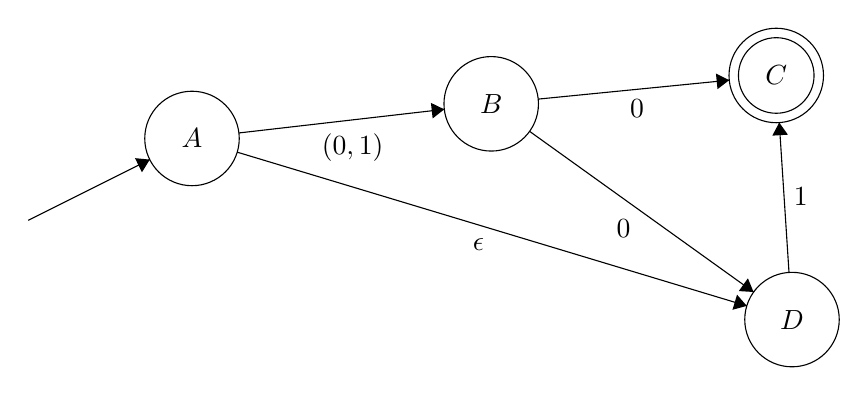
\begin{tikzpicture}[scale=0.2]
\tikzstyle{every node}+=[inner sep=0pt]
\draw [black] (16.1,-17.8) circle (3);
\draw (16.1,-17.8) node {$A$};
\draw [black] (35.1,-15.6) circle (3);
\draw (35.1,-15.6) node {$B$};
\draw [black] (53.2,-13.8) circle (3);
\draw (53.2,-13.8) node {$C$};
\draw [black] (53.2,-13.8) circle (2.4);
\draw [black] (54.2,-29.3) circle (3);
\draw (54.2,-29.3) node {$D$};
\draw [black] (5.7,-23) -- (13.42,-19.14);
\fill [black] (13.42,-19.14) -- (12.48,-19.05) -- (12.92,-19.95);
\draw [black] (37.54,-17.35) -- (51.76,-27.55);
\fill [black] (51.76,-27.55) -- (51.4,-26.68) -- (50.82,-27.49);
\draw (43.51,-22.95) node [below] {$0$};
\draw [black] (18.97,-18.67) -- (51.33,-28.43);
\fill [black] (51.33,-28.43) -- (50.71,-27.72) -- (50.42,-28.68);
\draw (34.29,-24.1) node [below] {$\epsilon$};
\draw [black] (19.08,-17.45) -- (32.12,-15.95);
\fill [black] (32.12,-15.95) -- (31.27,-15.54) -- (31.38,-16.53);
\draw (26.3,-17.45) node [below] {$(0,1)$};
\draw [black] (38.09,-15.3) -- (50.21,-14.1);
\fill [black] (50.21,-14.1) -- (49.37,-13.68) -- (49.47,-14.67);
\draw (44.36,-15.29) node [below] {$0$};
\draw [black] (54.01,-26.31) -- (53.39,-16.79);
\fill [black] (53.39,-16.79) -- (52.95,-17.62) -- (53.94,-17.56);
\draw (54.29,-21.51) node [right] {$1$};
\end{tikzpicture}
\end{center}

\end{document}
